\documentclass[12pt]{article}
\usepackage{amsmath}
%\usepackage[paperwidth=21cm, paperheight=29.8cm]{geometry}
\usepackage[angle=0,scale=1,color=black,hshift=-0.3cm,vshift=15cm]{background}
\usepackage{multirow}
\usepackage{enumerate}
\usepackage{changepage}

\backgroundsetup{contents={
{\bf \centering Statistics for Computing ------------------------ Lecture 15 ------------------------------------------ Solutions} }}


\setlength{\voffset}{-3cm}
\setlength{\hoffset}{-3.45cm}
\setlength{\parindent}{0cm}
\setlength{\textheight}{27cm}
\setlength{\textwidth}{19.7cm}

\pagestyle{empty}



\begin{document}



\framebox[1.02\textwidth]{
\begin{minipage}[t]{0.98\textwidth}
\begin{minipage}[t]{0.47\textwidth}
\subsection*{Question 1}
\begin{enumerate}[a)]
\item \quad \\[-1.45cm]
\begin{align*}
H_0:\quad \mu &= 2.5. \\
H_a:\quad \mu &\ne 2.5.
\end{align*}
\item The significance level is $\alpha=0.1$ $\Rightarrow$ $\alpha/2=0.05$ in each tail.\\[0.3cm]
    Small sample $\Rightarrow$ $t_{\,\nu,\,\alpha/2}$ required where the degrees of freedom are $\nu = n - 1 = 4 - 1 = 3$.\\[0.3cm]
    Thus, the critical values are $\pm t_{\,3,\,0.05} = \pm 2.353.$
\item \quad \\[-1.45cm]
\begin{center}
\begin{tabular}{|c|cccc|c|}
\multicolumn{2}{c}{}&&& \multicolumn{1}{c}{} & \multicolumn{1}{c}{$\sum$} \\[0.1cm]
\hline
&&&&&\\[-0.4cm]
$x$ & 2.53 & 2.55 & 2.54 & 2.24  & 9.86 \\[0.2cm]
$x^2$ & 6.4009 & 6.5025 & 6.4516 & 5.0176 &  24.3726 \\[0.1cm]
\hline
\multicolumn{6}{c}{}\\[-0.1cm]
\end{tabular}
\end{center}
\begin{align*}
\bar x &= \frac{\sum x}{n} = \frac{9.86}{4} = 2.465. \\[0.6cm]
s^2 &= \frac{\sum x^2 - n \, \bar x^2 }{n-1} = \frac{24.3726 - 4(2.465^2)}{3}\\[0.1cm] &\,\,\phantom{= \frac{\sum x^2 - n \, \bar x^2 }{n-1}} = 0.02256. \\[0.6cm]
s &= \sqrt{0.02256} = 0.1502.
\end{align*}
\end{enumerate}
\end{minipage}\hspace{0.055\textwidth}
\begin{minipage}[t]{0.47\textwidth}
\begin{enumerate}
\item[d)] Since the critical values are $t$ values, it is appropriate to label our test statistic $t$ rather than $z$ (although it is not essential).
    \begin{align*}
    t = \frac{\bar x - \mu_0}{\frac{s}{\sqrt{n}}} &= \frac{2.465 - 2.5}{\frac{0.1502}{\sqrt{4}}} \\[0.2cm]
    &= \frac{-0.035}{0.0751} \\[0.2cm]
    &=  -0.466.
    \end{align*}
\item[e)] Since $t=-0.466$ lies within the \emph{acceptance region}, $\pm 2.353$, there is not enough evidence to reject $H_0$ at the 10\% level of significance, i.e., we accept that $\mu = 2.5$.\\[0.4cm]
    The evidence suggests that the CPUs are performing as expected.
\end{enumerate}
\end{minipage}
\end{minipage}}\vspace{0.03\textwidth}



\framebox[1.02\textwidth]{
\begin{minipage}[t]{0.98\textwidth}
\begin{minipage}[t]{0.47\textwidth}
\subsection*{Question 2}
\begin{enumerate}[a)]
\item \quad \\[-1.45cm]
\begin{align*}
H_0:\quad \mu &\le 30. \\
H_a:\quad \mu &> 30.
\end{align*}
\item The significance level is $\alpha=0.01$. We do not divide by two since this is a one-tailed test; the rejection region is the \emph{upper tail} ($H_a: \mu > 30$).\\[0.3cm]
     Since $n>30$ the critical value is $z_{\,0.01} = 2.33$ \\ $\Rightarrow$ the rejection region is the area above $2.33$.\\[-1.3cm]
    \begin{center}
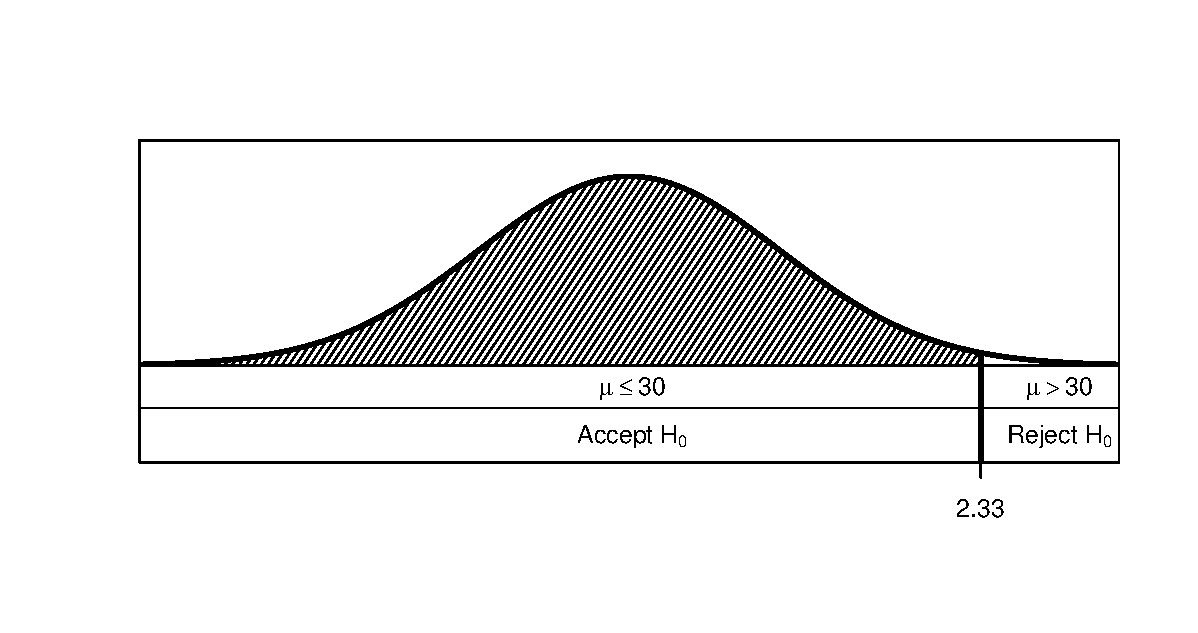
\includegraphics[width=0.98\textwidth, trim = 1.5cm 1.6cm 0.7cm 1.5cm, clip]{RejectRegion}
\end{center}
\end{enumerate}
\end{minipage}\hspace{0.055\textwidth}
\begin{minipage}[t]{0.47\textwidth}
\quad\\[-1cm]
\begin{enumerate}
\item[c)] We have $s^2 = 10$ $\Rightarrow$ $s = \sqrt{10}$.
    \begin{align*}
    \Rightarrow z = \frac{\bar x - \mu_0}{\frac{s}{\sqrt{n}}} &= \frac{32 - 30}{\frac{\sqrt{10}}{\sqrt{40}}} \\[0.2cm]
    &= \frac{2}{0.5} \\[0.2cm]
    &=  4.
    \end{align*}
\item[d)] Since $z=4$ is greater than $2.33$, we reject $H_0$ at the 1\% level of significance, i.e., we accept the alternative hypothesis that $\mu > 30$.\\[0.4cm]
    The evidence suggests that the CPUs are running hotter than expected.
\end{enumerate}
\end{minipage}
\end{minipage}}\vspace{0.03\textwidth}





\framebox[1.02\textwidth]{
\begin{minipage}[t]{0.98\textwidth}
\begin{minipage}[t]{0.47\textwidth}
\subsection*{Question 3}
\begin{enumerate}[a)]
\item \quad \\[-1.45cm]
\begin{align*}
H_0:\quad p &\le 0.5. \\
H_a:\quad p &> 0.5.
\end{align*}
\item The significance level is $\alpha=0.05$. Since this is a one-tailed test (and the alternative is pointing to the right tail) the critical value $z_{\,0.05} = 1.64$ \\ $\Rightarrow$ the rejection region is the area above $1.64$.
\item First calculate $\hat p = \frac{38}{65} = 0.5846$.
    \begin{align*}
    z = \frac{\hat p - p_0}{\sqrt{\frac{p_0\,(1-p_0)}{n}}} &= \frac{0.5846 - 0.5}{\sqrt{\frac{0.5\,(0.5)}{65}}}  \\[0.2cm]
    &= \frac{0.0846}{0.062} \\[0.2cm]
    &=  1.36.
    \end{align*}
Note that $p_0$ is used in the standard error calculation.
\end{enumerate}
\end{minipage}\hspace{0.055\textwidth}
\begin{minipage}[t]{0.47\textwidth}
\quad\\[-1cm]
\begin{enumerate}
\item[d)] Since $z=1.36$ is within the acceptance region (i.e., it is less than $1.64$), we accept $H_0$ at the 5\% level of significance.\\[0.4cm]
    The evidence suggests that more people prefer the old system.
\item[e)] This is a one-tailed test with a ``$>$'' in the alternative hypothesis:
    \begin{align*}
    \Rightarrow \text{p-value } = \Pr(Z > 1.36) = 0.0869.
    \end{align*}
    Therefore, while there is some evidence against $H_0$, it is not strong.\\[0.4cm]
    {\footnotesize(note that we would reject $H_0$ at the 10\% level)}
\end{enumerate}
\end{minipage}
\end{minipage}}\vspace{0.03\textwidth}








\end{document}



